\documentclass[aspectratio=169, numbering=fraction]{beamer}
\usetheme{metropolis}
\newcommand{\themename}{\textbf{\textsc{metropolis}}\xspace}

\usepackage{appendixnumberbeamer}
\usepackage{booktabs}
\usepackage{minted}
\usepackage{cleveref}
\usepackage[style=authortitle,backend=bibtex]{biblatex}
\usepackage[T1]{fontenc}
\usepackage{xspace}
\usepackage{graphicx}
\usepackage{tabularx}
\usepackage{caption}
\usepackage[super]{nth}
\usepackage{subcaption}
\captionsetup{labelformat=empty}
\subcaptionsetup{labelformat=empty}

\usepackage{tikz}
\usetikzlibrary{shapes.geometric, arrows.meta, positioning, calc, fit, shapes.multipart, shapes.callouts}

\usepackage{xcolor}

\renewcommand*{\bibfont}{\normalfont\small}
% Define custom colors to closely match the image
\definecolor{myyellow}{HTML}{FFEB3B}
\definecolor{mygreen}{HTML}{8BC34A}
\definecolor{myred}{HTML}{EF5350}
\definecolor{myblue}{HTML}{4FC3F7}
\definecolor{idxgray}{HTML}{9E9E9E} % Gray for indices

\setbeamertemplate{title page}{
    \advance\textwidth2cm
    \hsize\textwidth
    \columnwidth\textwidth
    \hspace*{-1cm}% the box is 2cm wider than the text area: center it on the slide
    \begin{minipage}[b][\paperheight]{\textwidth}
    \centering
    \vfill
    \ifx\inserttitle\@empty\else\usebeamertemplate*{title}\fi
    \ifx\insertsubtitle\@empty\else\usebeamertemplate*{subtitle}\fi
    \usebeamertemplate*{title separator}
    \ifx\beamer@shortauthor\@empty\else\usebeamertemplate*{author}\fi
    \ifx\insertdate\@empty\else\usebeamertemplate*{date}\fi
    \ifx\insertinstitute\@empty\else\usebeamertemplate*{institute}\fi
    \ifx\inserttitlegraphic\@empty\else\usebeamertemplate*{title graphic}\fi
    \vfill
    \vspace*{10mm}
    \end{minipage}
}
% center title and subtitle (metropolis defaults use \raggedright)
\setbeamertemplate{title}{
    \centering
    \linespread{1.0}%
    \inserttitle%
    \par%
    \vspace*{0.5em}
}
\setbeamertemplate{subtitle}{
    \centering
    \insertsubtitle%
    \par%
    \vspace*{0.5em}
}
% make the separator as wide as the title itself (capped at the text width)
\newsavebox{\titlerulebox}
\newlength{\titlerulewidth}
\setbeamertemplate{title separator}{%
    \sbox\titlerulebox{\usebeamerfont{title}\inserttitle}%
    \setlength{\titlerulewidth}{\wd\titlerulebox}%
    \ifdim\titlerulewidth>\textwidth\setlength{\titlerulewidth}{\textwidth}\fi
    \begin{tikzpicture}
        \fill[fg] (0,0) rectangle (\titlerulewidth, 0.4pt);
    \end{tikzpicture}%
    \par%
}
\setbeamertemplate{footline}{%
    \leavevmode
    \hfill
    \makebox[0.7cm][r]{% fixed width box, aligned right
        \parbox[c][0.7cm][c]{2cm}{% [c] = vertically center
        \scriptsize\hfill \insertframenumber{} / \inserttotalframenumber \hspace{2mm}
        }%
    }%
}
\AtBeginSection[]{}
\AtBeginSubsection[]{}

\title{Optimizing Breadth-First Search on the NVIDIA DGX Spark}
% \date{\today}
\date{}
\author[Fabio Missagia]{Student: Fabio Missagia \\ Supervisors: Flavio Vella, Thomas Pasquali, Jacopo Raffi}
\institute{Department of Information Engineering and Computer Science, University of Trento}
\titlegraphic{
\includegraphics[height=1cm]{images/logo.png} 
\includegraphics[height=1cm]{images/hicrest.png}
}

\newcommand{\bigO}[1]{\ensuremath{\mathcal{O}(#1)}}

\newenvironment{specialframe}
{
    \begingroup
    \advance\textwidth2cm % see beamerthemeGoettingen.sty for the number
    \hsize\textwidth
    \columnwidth\textwidth
    \begin{frame}[plain]
}
{
    \end{frame}
    \endgroup
}

\begin{document}

\maketitle

% ============================================================ 1. system (general)
\begin{frame}{NVIDIA DGX Spark: general properties}
  \vspace{0.7em}
  \small
  \begin{tabular}{ll}
    \toprule
    \textbf{Property} & \textbf{Value} \\
    \midrule
    System        & NVIDIA DGX Spark \\
    CPU           & 20 cores: 10$\times$ Cortex-X925 + 10$\times$ Cortex-A725 (aarch64) \\
    GPU           & NVIDIA GB10 --- compute capability 12.1 (\texttt{sm\_121}) \\
    Memory        & 128\,GB unified LPDDR5x, CPU--GPU coherent, $\sim$273\,GB/s \emph{shared} \\
    L2 cache      & 24\,MiB \\
    SMs           & 48 \\
    GPCs          & 4 (12 SMs each) --- \emph{measured, see next slides} \\
    Max grid      & 2\,147\,483\,647 $\times$ 65\,535 $\times$ 65\,535 \\
    \bottomrule
  \end{tabular}

  \vspace{0.4em}
  \footnotesize
  One \emph{physical} memory pool, hardware coherent: a kernel dereferences a plain
  \texttt{malloc()} pointer with no \texttt{cudaMemcpy}. $\sim$273\,GB/s is an order of
  magnitude below datacenter HBM, like H100 ($\sim$2.0\,TB/s).

\end{frame}

% ============================================================ 2. system (per SM)
\begin{frame}{NVIDIA DGX Spark: per-SM properties}
  \vspace{0.7em}
  \small
  \begin{tabular}{ll}
    \toprule
    \textbf{Property} & \textbf{Value} \\
    \midrule
    Max threads / block                  & 1024 \\
    Max threads / SM                     & 1536 (48 warps) \\
    Max blocks / SM                      & 24 \\
    Registers / SM                       & 65\,536 \\
    \midrule
    Unified L1 + shared memory           & 128\,KiB \\
    Max shared memory / SM               & 102\,400\,B (100\,KiB) \\
    Default shared memory / block        & 49\,152\,B (48\,KiB) \\
    Max shared memory / block (opt-in)   & 101\,376\,B (99\,KiB) \\
    Reserved shared memory / block       & 1\,024\,B \\
    %\midrule
    %SM clock (observed under load)       & 2.40\,GHz \\
    \bottomrule
  \end{tabular}
  
  \vspace{0.8em}
  \footnotesize
  L1 and shared memory are the \emph{same} 128\,KiB SRAM, split by a configurable
  carveout: shared memory is bought at the cost of L1.
  
\end{frame}

% ============================================================ 3. clusters: concept
\begin{frame}{Thread block clusters (compute capability 9.0+)}
  \vspace{0.7em}
  \footnotesize
  An optional level between block and grid:
  \begin{itemize}\itemsep1pt
    \item \textbf{adjacent thread blocks} are grouped into clusters
    \item guaranteed to be \textbf{co-scheduled simultaneously inside one GPC}
    \item any thread block can address \textbf{any peer's shared memory} --- loads, stores and
    \emph{atomics} ride an \textbf{SM-to-SM} interconnect, not L2/DRAM $\Rightarrow$ \textbf{DSMEM}
    \item \textbf{co-residency} is guaranteed
    \item hardware barrier across blocks: \texttt{cluster.sync()}
  \end{itemize}
  \vspace{0.5em}
  \centering
  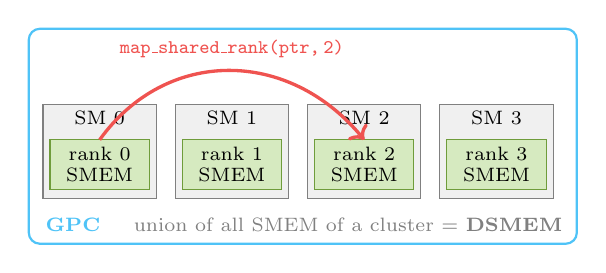
\begin{tikzpicture}[scale=0.6, every node/.style={font=\scriptsize}]
    \draw[rounded corners, thick, myblue] (-0.3,-0.95) rectangle (11.3,3.6);
    \node[anchor=south west, myblue, font=\scriptsize\bfseries] at (-0.15,-0.9) {GPC};
    \foreach \i/\x in {0/0, 1/2.8, 2/5.6, 3/8.4} {
      \draw[fill=gray!12, draw=gray] (\x,0) rectangle (\x+2.4,2.0);
      \node at (\x+1.2,1.72) {SM \i};
      \draw[fill=mygreen!35, draw=mygreen!80!black] (\x+0.15,0.2) rectangle (\x+2.25,1.25);
      \node at (\x+1.2,0.95) {rank \i};
      \node at (\x+1.2,0.5) {SMEM};
    }
    \draw[->, very thick, myred] (1.2,1.25) .. controls (2.6,3.2) and (5.2,3.2) .. (6.8,1.25);
    \node[myred, anchor=south] at (4.0,2.78) {\texttt{map\_shared\_rank(ptr,\,2)}};
    \node[anchor=south east, gray] at (11.2,-0.9) {union of all SMEM of a cluster $=$ \textbf{DSMEM}};
  \end{tikzpicture}

\end{frame}

% ============================================================ 4. clusters on GB10
\begin{frame}{Thread block clusters on the DGX Spark}
  \vspace{0.7em}
  \centering
  \small
  \begin{tabular}{lcc}
    \toprule
    \textbf{Measurement}        & \textbf{portable} & \textbf{with opt-in} \\
    \midrule
    Cluster Size       & 8              & 12 \\
    \bottomrule
  \end{tabular}

  \vspace{0.6em}
  \raggedright
  \footnotesize
  \begin{itemize}\itemsep3pt
    \item \textbf{8} is the maximum CUDA guarantees \emph{portably} on any
          cluster-capable GPU --- code using it runs anywhere.
    \item \textbf{12} is \emph{this hardware's} real maximum, unlocked per kernel with
          \texttt{cudaFuncAttributeNonPortableClusterSizeAllowed} --- at the price of
          code that is no longer portable. Above 12: \emph{cluster misconfiguration}.
    \item \texttt{cudaOccupancyMaxPotentialClusterSize} is \textbf{per kernel}, not a
          device constant: the same kernel answers 8 before the opt-in and 12 after.
    \item 12 is \emph{usable}, not merely launchable: DSMEM verified across all 12 ranks
          with a ring test (rank $r$ reads rank $r{+}1 \bmod n$).
  \end{itemize}

\end{frame}

% ============================================================ 5a. GPC method
\begin{frame}{How many GPCs?}
  \vspace{0.7em}
  \footnotesize
  \textbf{Problem.} No CUDA attribute exposes the GPC count or the SM-to-GPC mapping.

  \vspace{0.6em}
  \textbf{Idea.} Exploit the one guarantee available: \emph{all blocks of a cluster are
  co-scheduled in a single GPC}. So the SMs hosting one cluster are provably all
  in the \emph{same} GPC.

  \vspace{0.6em}
  \textbf{Method.} A \emph{single} launch of 4 clusters $\times$ 12 blocks.
  \begin{itemize}\itemsep3pt
    \item every block reads the \texttt{\%smid} register and reports the SM it
          ran on and the cluster it belongs to
    \item 52\,KB of shared memory per block forces one block per SM, so a
          12-block cluster covers 12 \emph{distinct} SMs
    \item cluster size 12 $=$ one GPC's SM count, so 4 clusters cover all 48 SMs
          exactly once and \textbf{each cluster \emph{is} a GPC} --- read the
          mapping off directly
    \item tried many trials, but the result is always the same and all 48 SMs
          are observed every time, so one launch is enough
  \end{itemize}

\end{frame}

% ============================================================ 5b. GPC result
\begin{frame}{GPC topology: 4 GPCs $\times$ 12 SMs}
  \footnotesize
  \textbf{Example:}\vspace{-0.3em}

  \centering
  \begin{tabular}{ll}
    \toprule
    \textbf{GPC} & \textbf{SM ids} \\
    \midrule
    GPC 0 & \texttt{0\ \ 1\ \ 8\ \ 9\ 16\ 17\ 24\ 25\ 32\ 33\ 40\ 41} \\
    GPC 1 & \texttt{2\ \ 3\ 10\ 11\ 18\ 19\ 26\ 27\ 34\ 35\ 42\ 43} \\
    GPC 2 & \texttt{4\ \ 5\ 12\ 13\ 20\ 21\ 28\ 29\ 36\ 37\ 44\ 45} \\
    GPC 3 & \texttt{6\ \ 7\ 14\ 15\ 22\ 23\ 30\ 31\ 38\ 39\ 46\ 47} \\
    \bottomrule
  \end{tabular}

  \raggedright
  \footnotesize
  \vspace{0.2em}
  \textbf{Derived and verified:}\vspace{-0.3em}
  \begin{itemize}\itemsep0pt
    \item \texttt{TPC = smid/2}, \quad \texttt{GPC = (smid/2) \% 4}
    \item 24 TPCs of 2 SMs, 6 TPCs per GPC, round-robin across GPCs
  \end{itemize}

  \textbf{Three independent cross-checks:}\vspace{-0.3em}
  \begin{itemize}\itemsep0pt
    \item 4 clusters of 12 \emph{distinct} SMs, 48 SMs observed, none twice
    \item $4 \times 12 = 48$ matches \texttt{multiProcessorCount}
    \item the largest launchable cluster (12) \emph{equals} one GPC's SM count
  \end{itemize}
\end{frame}

% ============================================================ 7. latency
\begin{frame}{Latency Benchmark -- Random pChase}
  \vspace{0.2em}
  \footnotesize
  Dependent random pointer chase, 16\,384 steps, one thread, median of 101 reps.
  \vspace{-0.5em}
  \begin{itemize}\itemsep0pt
    \item \textbf{Sattolo cycle.} One random cycle over all elements: no short cycles, nothing for a prefetcher.
    \item \textbf{Dependency defeats overlap.} Load $i{+}1$ needs the value of load $i$: pure latency, no MLP.
  \end{itemize}

  \vspace{0.2em}
  \centering
  \begin{tabular}{lccc}
    \toprule
    \textbf{Placement} & \textbf{GB10 (cy)} & \textbf{ns} & \textbf{H800 (cy)}$^{\star}$ \\
    \midrule
    L1 Cache                                     & 43.2      & 17.9      & 32.0 \\
    SMEM                 & 32.9 & 13.7 & 29.0 \\
    SMEM, via DSMEM API      & 36.9 & 15.3 & 33.0 \\
    DSMEM      & 180-211 & 75-88 & 181-213 \\
    L2 Cache                                     & 340.1     & 141.7     & 264--502 \\
    DRAM                                       & 965.8     & 401.6     & 656 \\
    \bottomrule
  \end{tabular}

  \vspace{0.2em}
  {\tiny\color{gray} $^{\star}$ Luo et al., arXiv:2501.12084 --- Hopper H800, same p-chase method}

  \vspace{0.2em}
  \raggedright
  \scriptsize
  \textbf{Why does SMEM via DSMEM cost 4 more cycles?} \texttt{map\_shared\_rank} returns a generic pointer, so the load compiles to \texttt{LD} (address space resolved by hardware on every access) instead of \texttt{LDS} (a plain shared-memory load).
\end{frame}

\begin{frame}{Latency Benchmark -- Random pChase}
  \vspace{0.2em}
  \footnotesize
  Dependent random pointer chase, 16\,384 steps, one thread, median of 101 reps.
  \vspace{-0.5em}
  \begin{itemize}\itemsep0pt
    \item \textbf{Sattolo cycle.} One random cycle over all elements: no short cycles, nothing for a prefetcher.
    \item \textbf{Dependency defeats overlap.} Load $i{+}1$ needs the value of load $i$: pure latency, no MLP.
  \end{itemize}

  \centering
  \begin{figure}
    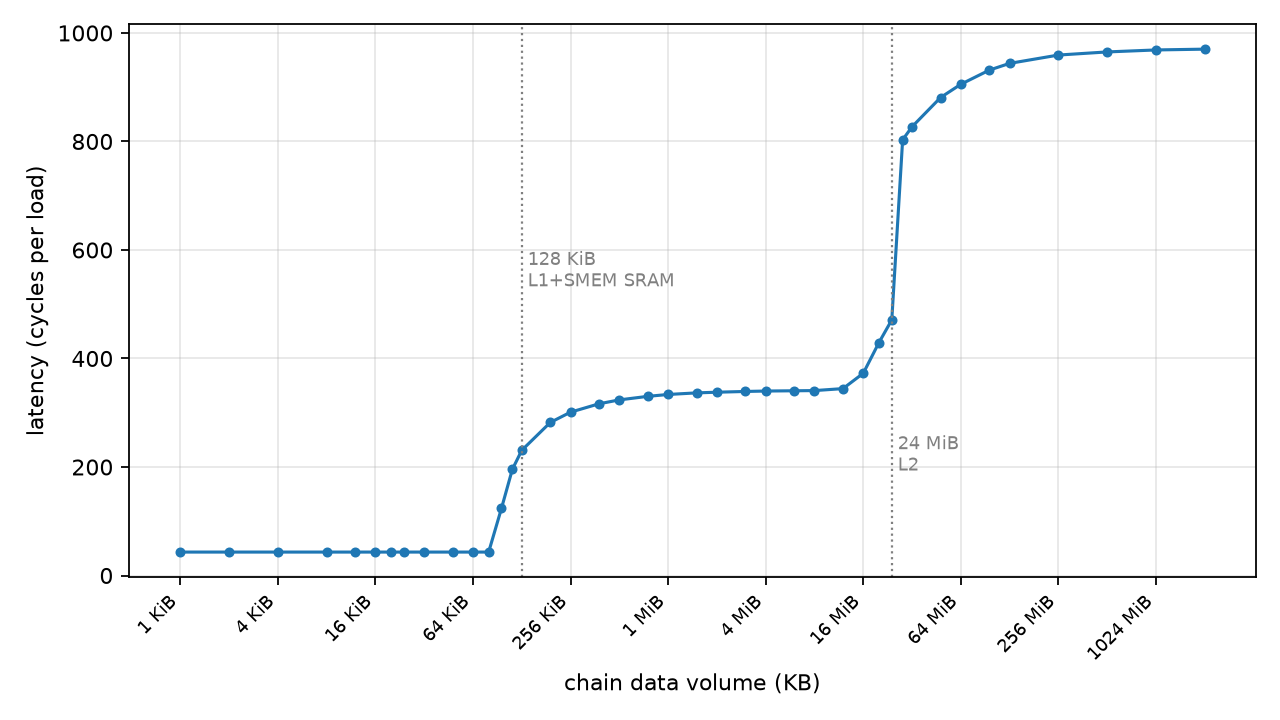
\includegraphics[width=0.7\linewidth]{images/chain_latency.png}
  \end{figure}
\end{frame}

\begin{frame}{Latency Benchmark -- Random pChase}
  \vspace{0.2em}
  \footnotesize
  Same chase, but thread 0 of rank 0 accesses a \emph{peer} block's SMEM at rank distance $d$, median of 101 reps.

  \vspace{0.1em}
  \centering
  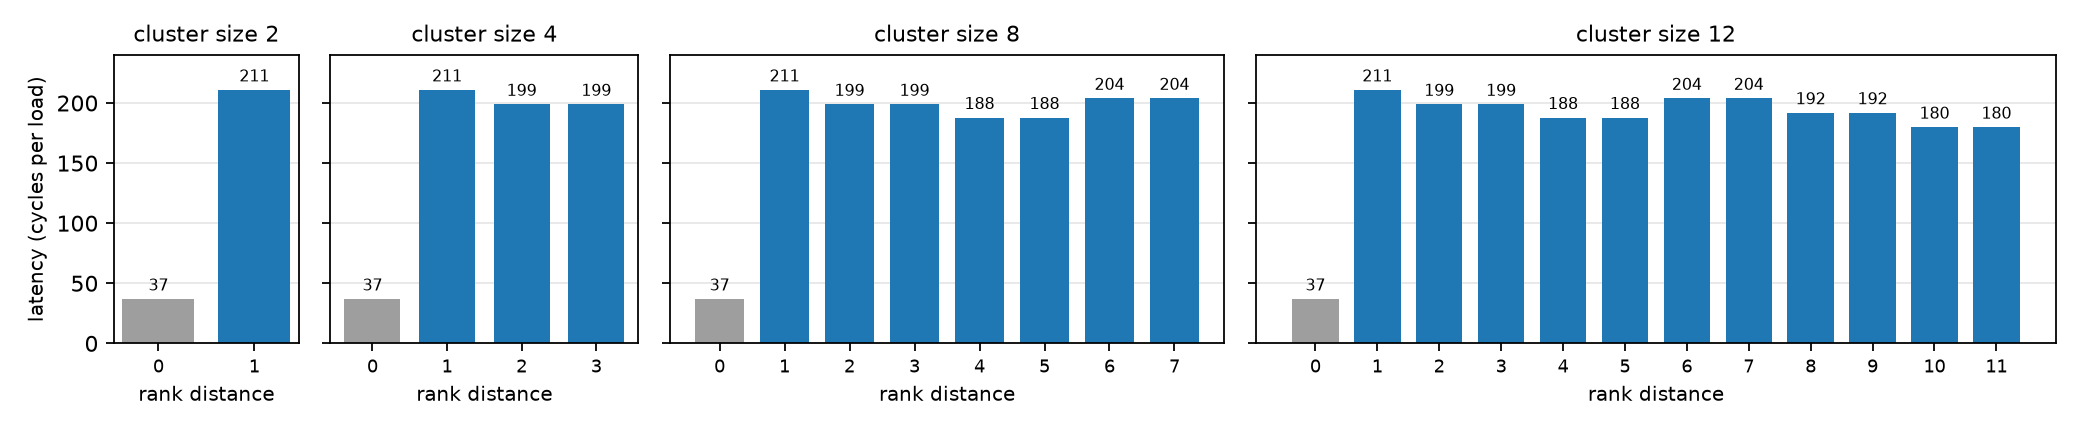
\includegraphics[width=\linewidth]{images/dsmem-distance.png}

  \vspace{0.1em}
  \raggedright
  \begin{itemize}\itemsep1pt
    \item \textbf{A genuine SM-to-SM path.} A remote access costs about \emph{half} an L2 hit and a \emph{fifth}
          of DRAM.
    \item \textbf{Flat across the cluster.} 210.9\,cy at distance 1, identically at cluster
          sizes 2, 4, 8 and 12. Not monotone in distance: ranks pair up
          $\{2,3\},\{4,5\},\dots$ --- the two SMs of one TPC.
    \item \textbf{Independently confirmed.} H800 agrees within a few cycles; since GB10's L2 and
          DRAM are \emph{slower} than Hopper's while its fabric is not, DSMEM's advantage is \emph{larger} here.
  \end{itemize}

\end{frame}

\begin{frame}{Latency Benchmark -- Linear pChase}
  \vspace{0.3em}
  \scriptsize
  Same chase, but element $i$ points to $i+s$, $s = 4\,\mathrm{B} \ldots 4\,\mathrm{KiB}$.
  Dashed = random chase (previous slide).

  \vspace{0.5cm}
  \begin{columns}
    \begin{column}{0.7\textwidth}
      \centering
      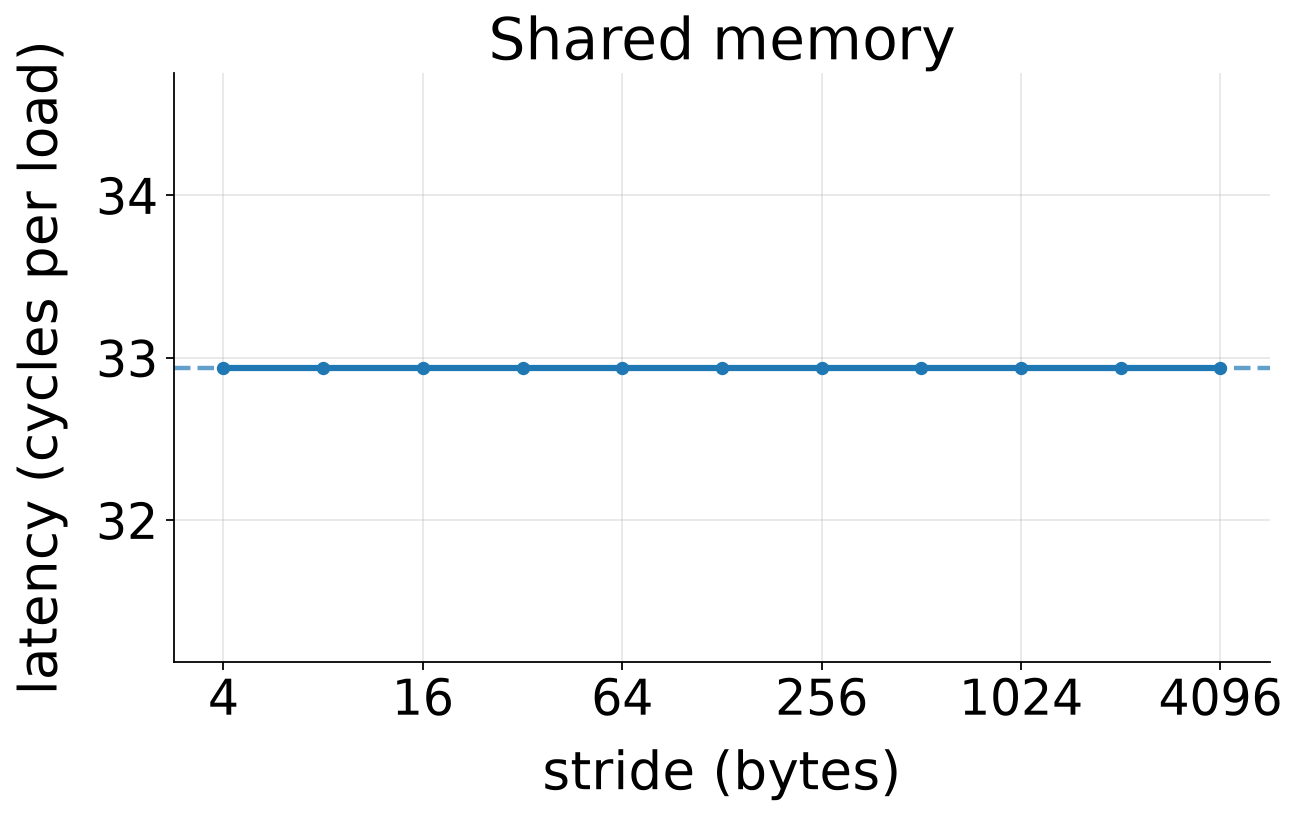
\includegraphics[width=0.49\linewidth]{images/stride-smem.png}\hfill
      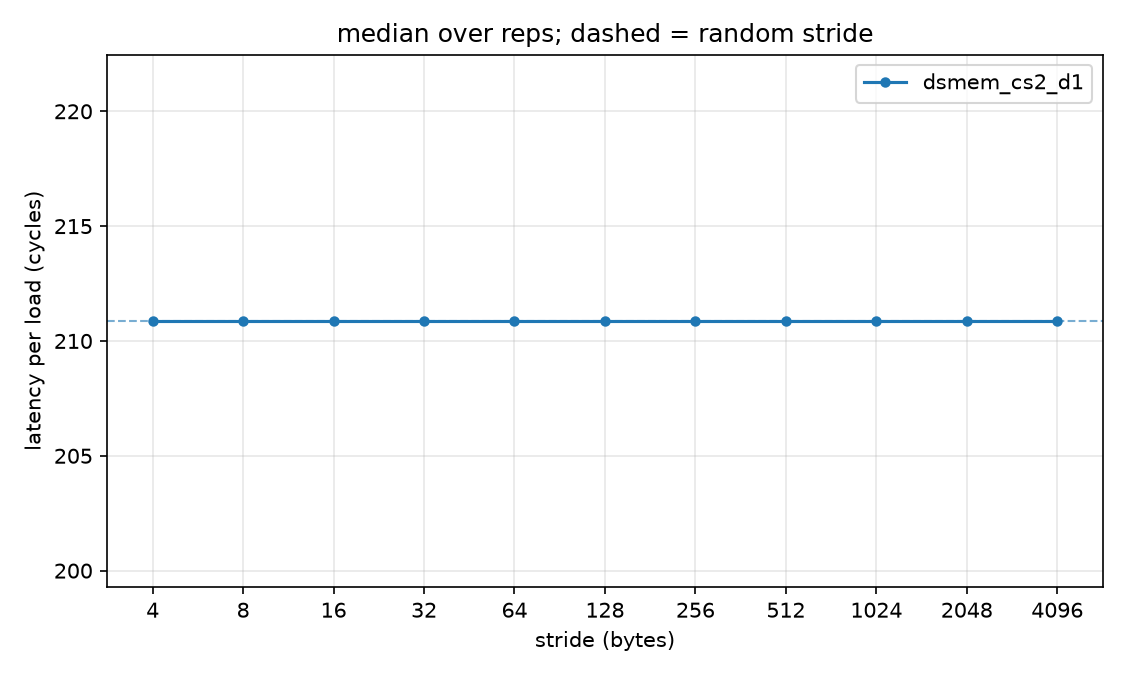
\includegraphics[width=0.49\linewidth]{images/stride-dsmem-c2-d1.png}\\[2pt]
      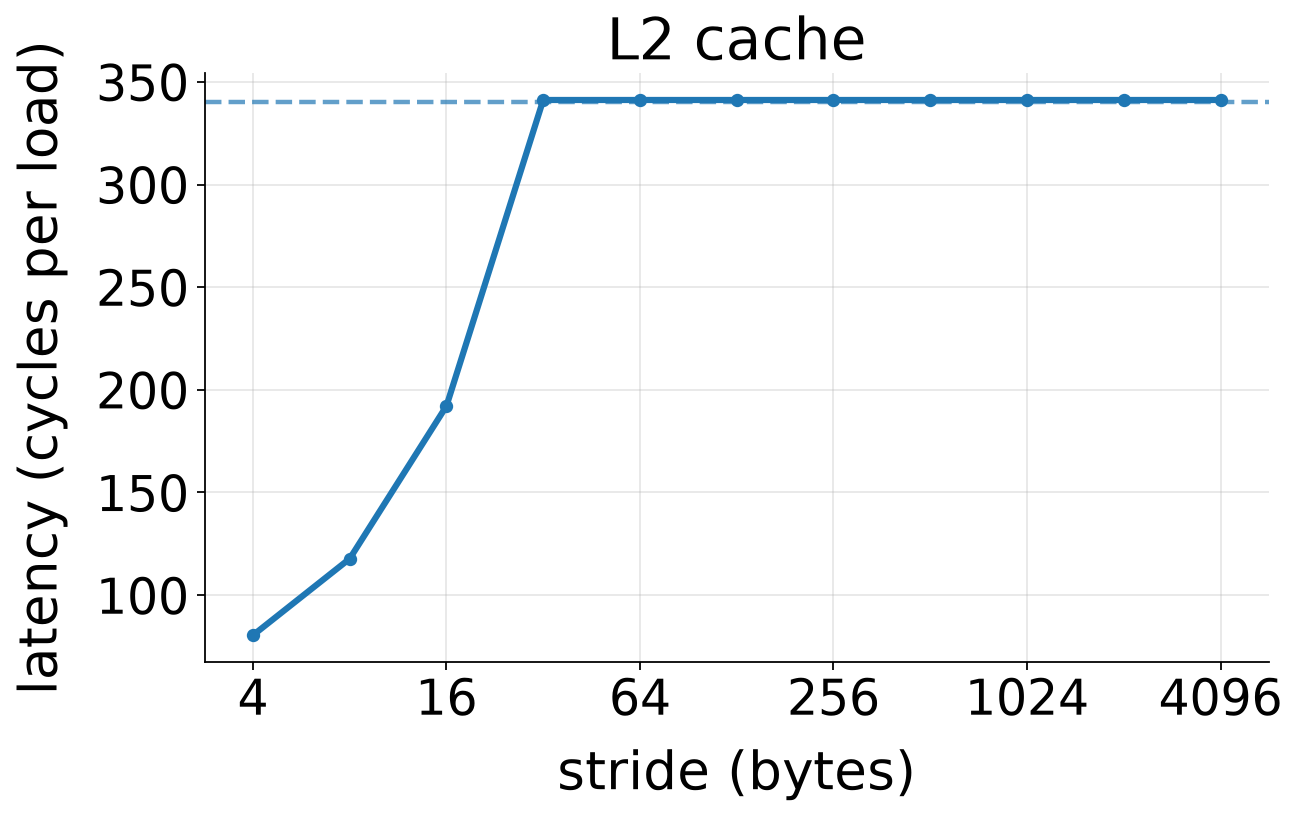
\includegraphics[width=0.49\linewidth]{images/stride-l2.png}\hfill
      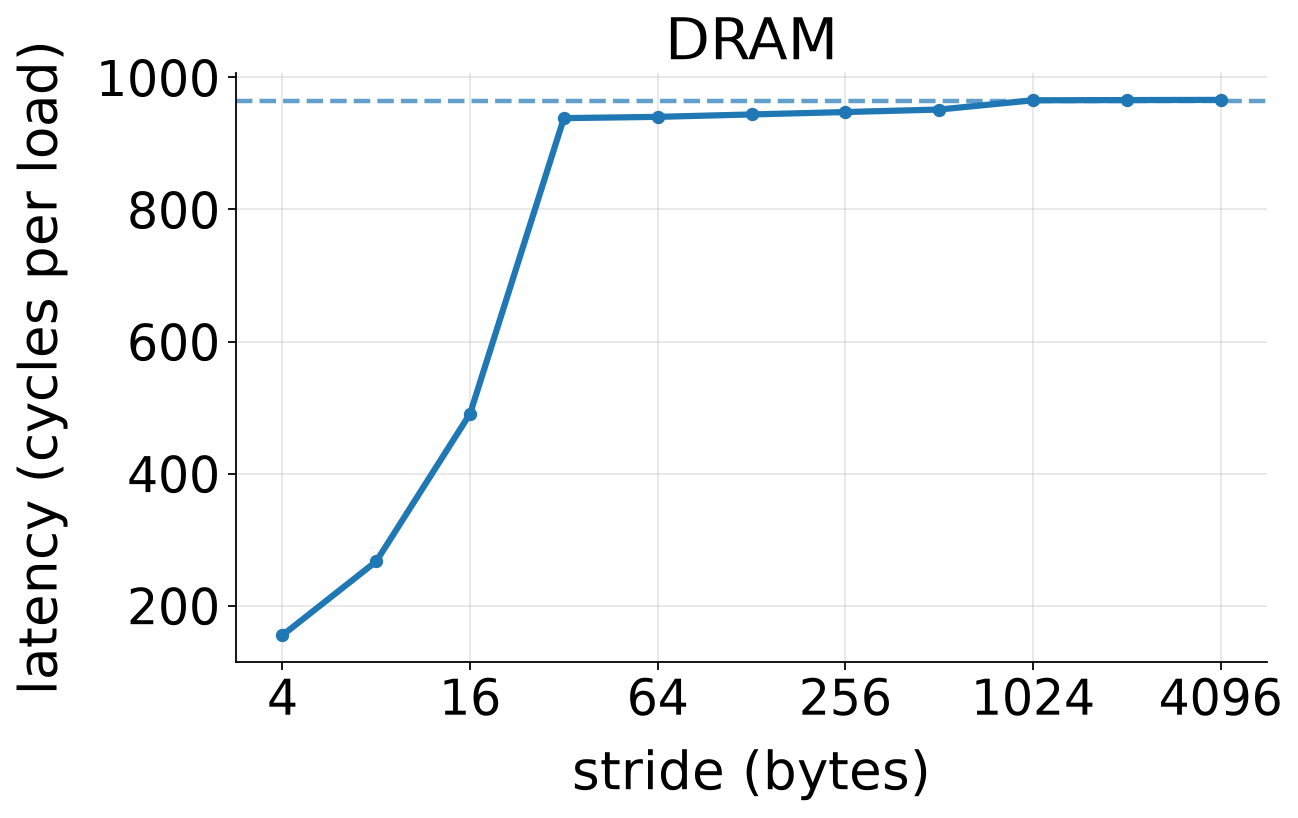
\includegraphics[width=0.49\linewidth]{images/stride-dram.png}
    \end{column}
    \begin{column}{0.4\textwidth}
      \begin{itemize}\itemsep2pt
        \item \textbf{SMEM/DSMEM are pattern-blind}
        \item \textbf{L2/DRAM see only the 32\,B sector} $k = 32/s$ loads share one
              L1 fill, $(T + (k-1)\cdot 43.2)/k$ gives 80/118/192\,cy (L2) and
              155/266/490\,cy (DRAM) --- as measured.
        \item \textbf{No hardware prefetcher:} from 32\,B on, linear $=$ random.
      \end{itemize}
    \end{column}
  \end{columns}
\end{frame}

% ============================================================ 6. cluster residency cap
\begin{frame}{Clusters are not free}
  \vspace{0.5em}
  \footnotesize
  The moment a launch carries a cluster dimension, the device holds \textbf{2 blocks
  per SM at most (96 in total), whatever the block size.}

  \vspace{0.5em}
  \centering
  \begin{tabular}{lcccc}
    \toprule
    \textbf{blockDim} & \textbf{total blocks} & \textbf{total blocks} & \textbf{penalty} & \textbf{occupancy} \\
     & \textbf{(unclustered)} & \textbf{(clustered)} & & \textbf{(clustered)} \\
    \midrule
    64   & 1152 & 96 & \textbf{12$\times$} & 8\% \\
    128  & 576  & 96 & 6$\times$           & 17\% \\
    256  & 288  & 96 & 3$\times$           & 33\% \\
    512  & 144  & 96 & 1.5$\times$         & \textbf{67\%} \\
    1024 & 48   & 48 & none                & 67\% \\
    \bottomrule
  \end{tabular}

  \vspace{0.6em}
  \raggedright
  \begin{itemize}\itemsep1pt
    \item \textbf{Confirmed two independent ways:} \texttt{cudaOccupancyMaxActiveClusters}, and a test in which every block must observe all the others before a timeout.
    \item \textbf{Didn't found anything about this on the web...}
  \end{itemize}

\end{frame}

\begin{frame}{Clusters are not free}
  \vspace{0.5em}
  \footnotesize
  The cap also moves with the \emph{shared memory} a block requests. Past
  ${\sim}50$\,KiB only one block fits per SM, so the device holds 48.

  \vspace{0.4em}
  \centering
  \begin{tabular}{lccccc}
    \toprule
    \textbf{SMEM / block} & \textbf{cs = 1} & \textbf{cs = 2} & \textbf{cs = 4} & \textbf{cs = 8} & \textbf{cs = 12} \\
    \midrule
    0            & 96 & 96 & 96 & 96          & 96 \\
    32\,KiB      & 96 & 96 & 96 & 96          & 96 \\
    50\,KiB      & 48 & 48 & 48 & \textbf{32} & 48 \\
    99\,KiB      & 48 & 48 & 48 & \textbf{32} & 48 \\
    \bottomrule
  \end{tabular}

  \vspace{0.3em}
  {\scriptsize total resident blocks device-wide (48 SMs), \texttt{cs} = cluster size}

  \vspace{0.6em}
  \raggedright
  \begin{itemize}\itemsep1pt
    \item A cluster never spans a GPC, and a GPC has 12 SMs. One cluster of 8 leaves 4 SMs free --- too few for a second --- so each of the 4 GPCs runs one cluster and strands 4 SMs: $4 \times 8 = 32$, a third of the GPU idle.
    \item \textbf{12 and 6 tile the machine exactly}; 8, the \emph{portable}
          maximum, does not.
  \end{itemize}

\end{frame}

% \begin{frame}{TODO}
%   \begin{itemize}\itemsep1pt\small
%     \item quanto si fa fatica a fare lo scheduling in concorrenza con altri processi (che impatto ha lo scheduler)
%     \item un altra versione del benchmark in cui non è solo il thread 0 a fare il chase, ma tutti i thread del cluster fanno il chase in concorrenza, e si misura quanto aumenta la latenza per via dello scheduling.
%     \item cosa succede se invece di una random chase usiamo una linear chase, cioè un buffer in cui ogni elemento punta al successivo, e l'ultimo punta al primo. In questo caso il prefetcher dovrebbe essere in grado di anticipare le richieste e ridurre la latenza.
%     \item provare a usare stride-n
%     \item tenersi la varianza, prendi le run, emetti tutti i numeri, passare i parametri da cli, ogni programma una casistica

%     \item slides con disegnini, come funziona l'accesso, il warmup
%     \item fare grafici
%     \item usare spatzman riproducibilità, come si fa a garantire che il benchmark sia riproducibile
%   \end{itemize}
% \end{frame}

\begin{frame}{Latency Benchmark -- Many Threads}
\vspace{0.2em}
  \centering
  \begin{figure}
    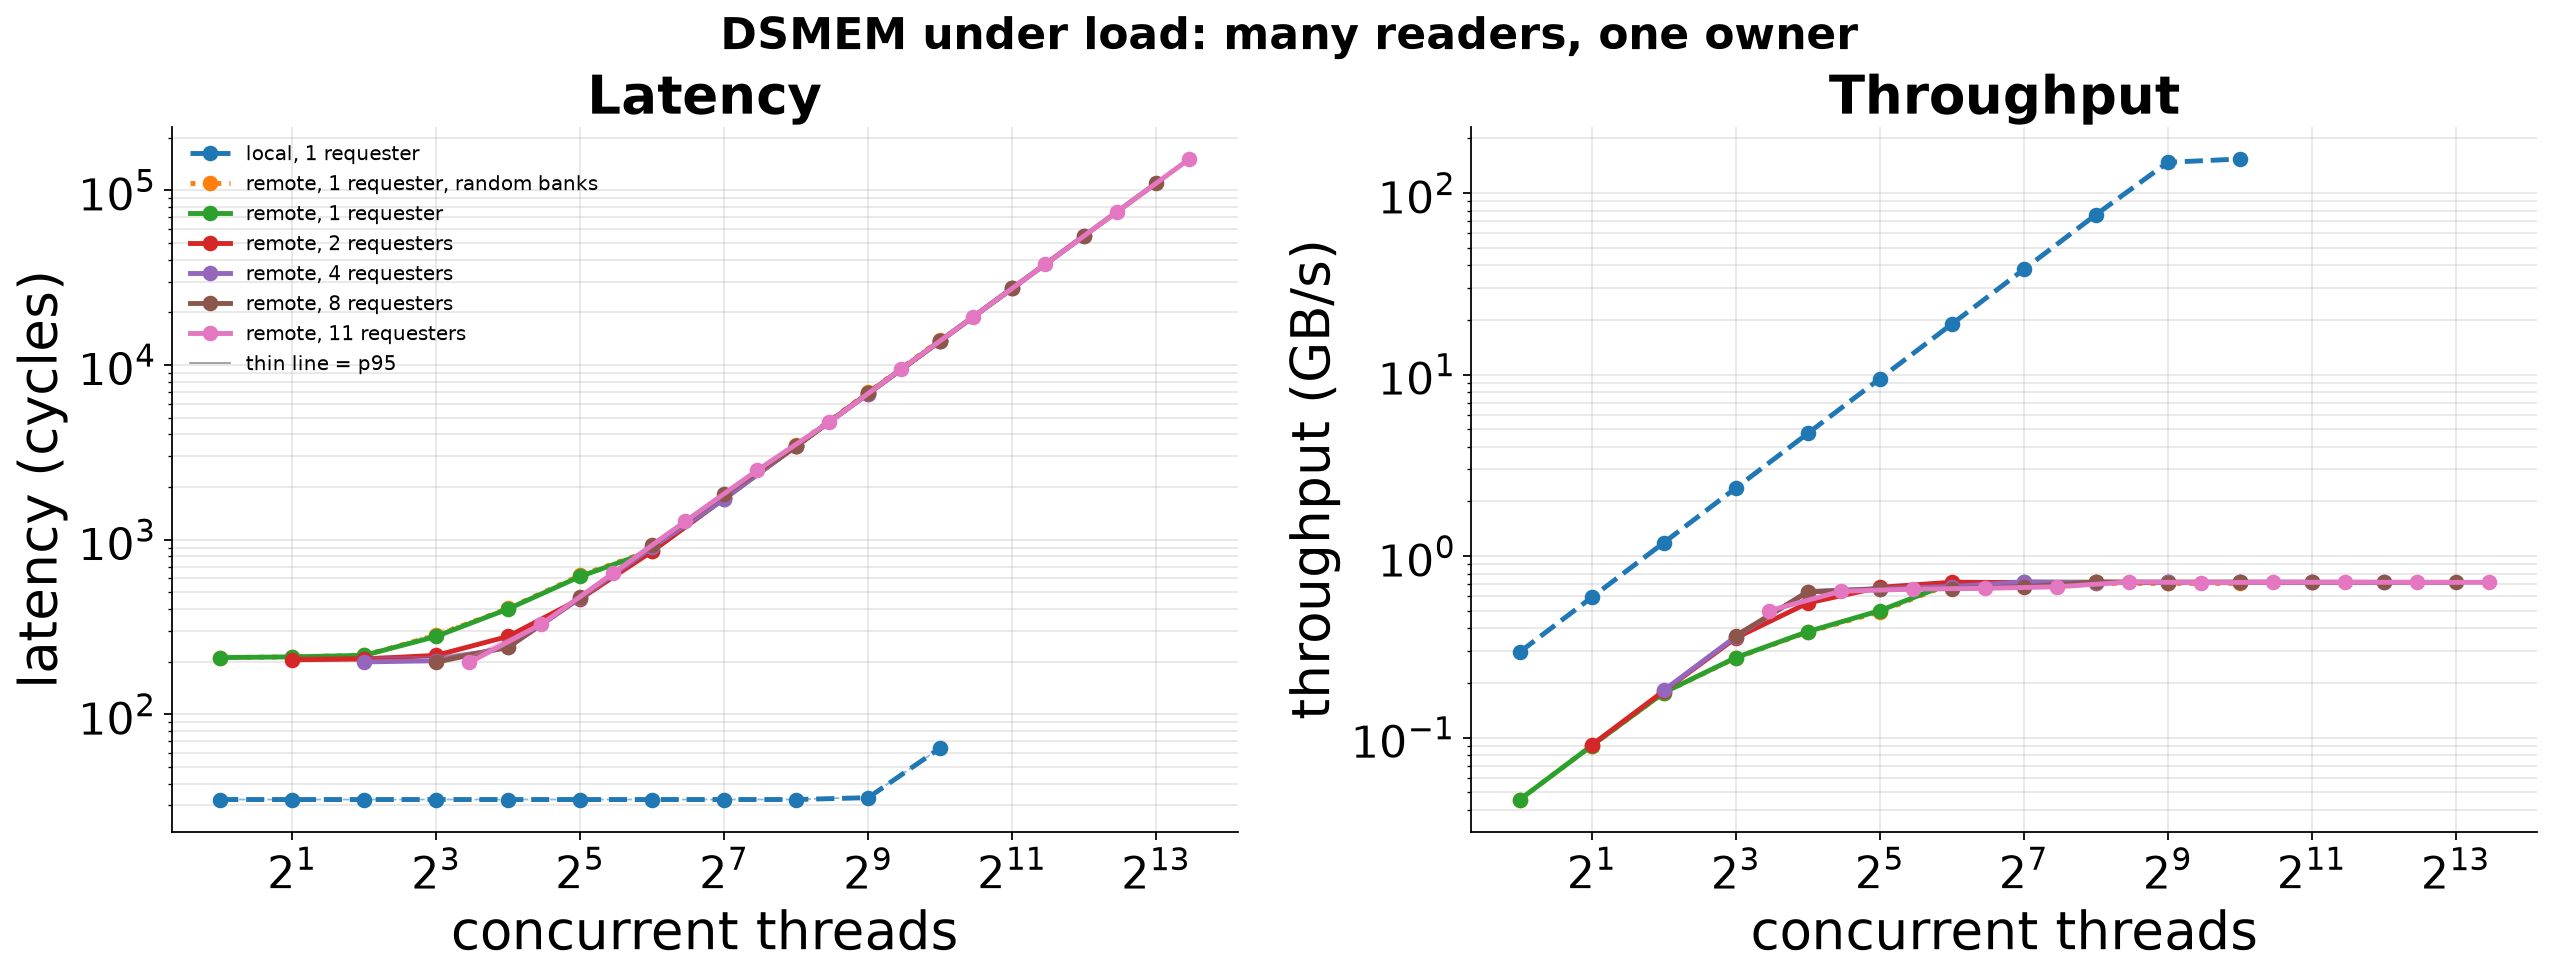
\includegraphics[width=0.99\linewidth]{images/loaded_latency.png}
  \end{figure}
\end{frame}

\begin{frame}{What's next?}
  \footnotesize
  \begin{enumerate}\itemsep0pt
    \item \textbf{Characterization of DSMEM}
      \begin{itemize}\scriptsize\itemsep0pt
        \item Performance characterization and impact of DSMEM
        \item Limitations and assumptions of the DSMEM programming paradigm
        \item Theoretical upper bounds on performance improvements
        \item Applicability: algorithms that can and cannot exploit DSMEM
      \end{itemize}
    \item \textbf{State-of-the-art GPU-accelerated BFS}
      \begin{itemize}\scriptsize\itemsep0pt
        \item Graph partitioning strategies
        \item Work-stealing techniques
        \item Data types and data structures for high-performance BFS
      \end{itemize}
    \item \textbf{BFS implementation based on DSMEM}
      \begin{itemize}\scriptsize\itemsep0pt
        \item Algorithm design informed by (1) and (2)
        \item Graph partitioning (probably 2D) and work stealing
        \item Integration of \emph{mxint} (micro-scaling integer type), if worthwhile
        \item Performance evaluation; limitations and future directions
      \end{itemize}
  \end{enumerate}
\end{frame}

\end{document}